\documentclass{beamer}
\usetheme{metropolis}
\setbeamercovered{transparent}

\usepackage{amsmath, amssymb, amsthm}
\usepackage{graphicx}
\usepackage{epstopdf}
\usepackage[scr]{rsfso}
\usepackage{forloop}

\def\C{\mathbb{C}}
\def\R{\mathbb{R}}
\def\Q{\mathbb{Q}}
\def\Z{\mathbb{Z}}
\def\N{\mathbb{N}}

\title{
    The Stone-Weierstrass Theorem
}
\subtitle{
    Approximating continuous functions by smooth functions
    \vspace{-2em}
}
\author{Satvik Saha}
\institute{
    Summer Programme \\
    Indian Institute of Science Education and Research, Kolkata
}
\date{\today}

\begin{document}
    \maketitle

    \section{Approximation in metric spaces}

    \begin{frame}{Approximation}
    \begin{center}
        The object $\alpha$ approximates $\beta$, to some degree of accuracy
        $\epsilon$.
        \[\updownarrow\]
        \[
            d(\alpha, \beta) < \epsilon
        \]
        \[\updownarrow\]
        $\alpha$ lies within a narrow region centred at $\beta$.
    \end{center}
    \end{frame}

    \begin{frame}{Approximation}
    \begin{center}
        The sequence $\{\alpha_n\}$ converges to $\beta$.
        \[\updownarrow\]
        Given any $\epsilon$, there exists $n_0$ such that for all $n \geq n_0$,
        \[
            d(\alpha_n, \beta) < \epsilon
        \]
        \[\updownarrow\]
        Every neighbourhood of $\beta$ contains some tail of $\{\alpha_n\}$.
    \end{center}
    \end{frame}

    \begin{frame}{Approximation}
        \[
            1 - \frac{1}{3} + \frac{1}{5} - \frac{1}{7} + \dots \to \frac{\pi}{4}
        \] 

        \\~\\

        \[
            x - \frac{1}{3}x^3 + \frac{1}{5}x^5 - \frac{1}{7}x^7 + \dots \to
            \arctan{x}
        \] 

        \\~\\

        \begin{center}
            This series converges \emph{uniformly} on $[-1, +1]$.
        \end{center}
    \end{frame}

    \begin{frame}{Approximating $\arctan{x}$}
        \begin{figure}
            \centering
            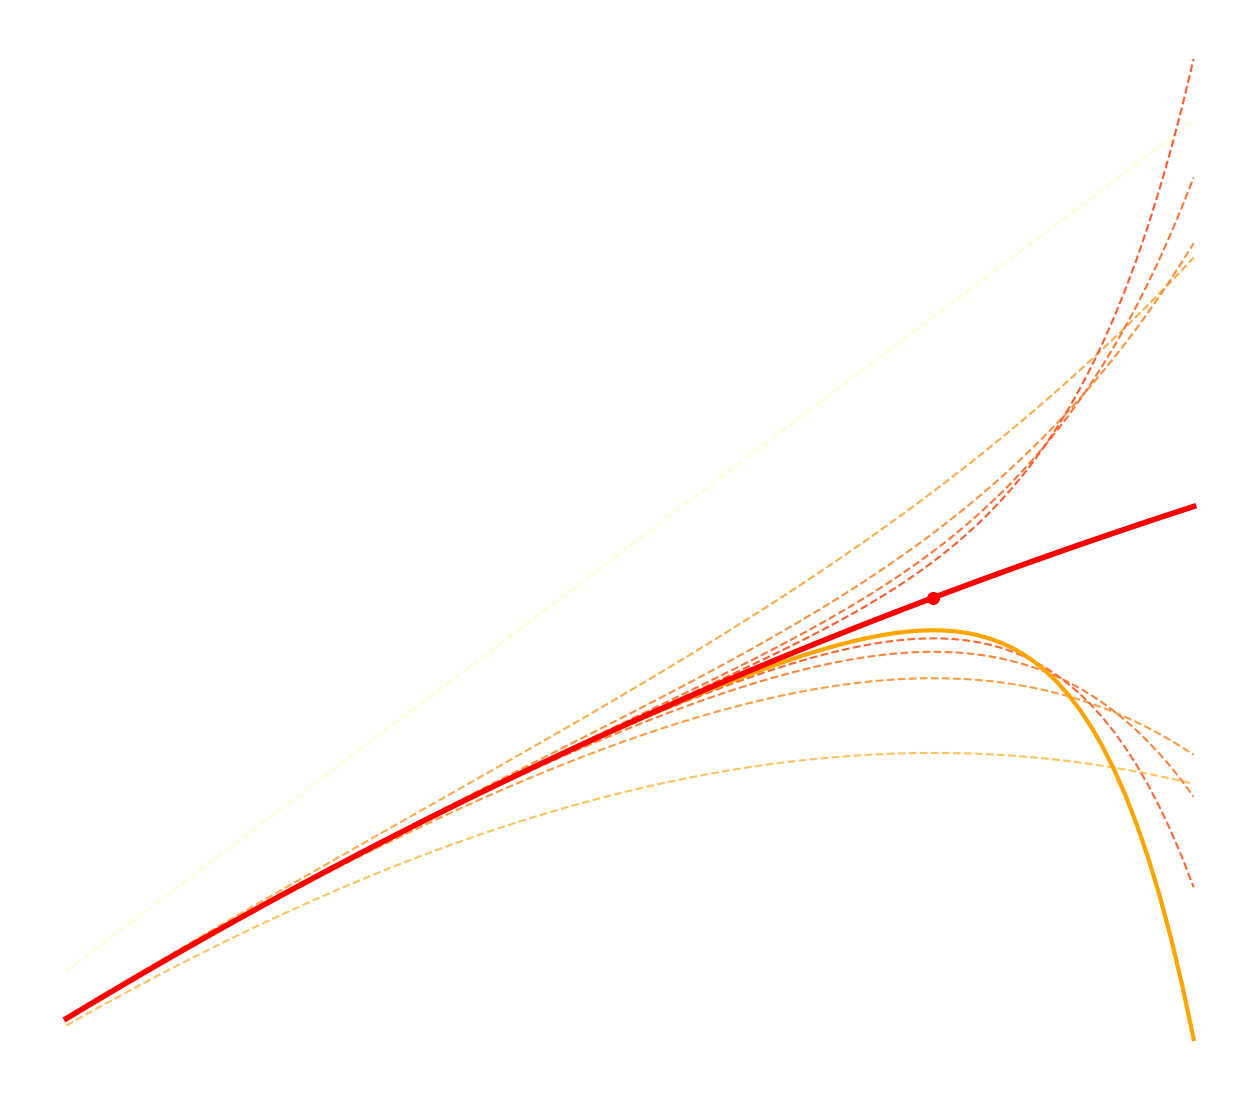
\includegraphics[width=0.9\textwidth]{./img/arctan.png}
            \label{fig:arctan}
        \end{figure}
    \end{frame}

    \begin{frame}{Integrating a uniformly convergent series}
        A power series converges uniformly on its interval of convergence.

        \begin{align*}
            \cos{x} &= \sum_{n = 0}^\infty (-1)^n \frac{x^{2k}}{(2k)!} \\
            \sin{x} &= \sum_{n = 0}^\infty (-1)^n \frac{x^{2k + 1}}{(2k + 1)!}
        \end{align*}

        \\~\\

        \[
            \int_a^b \cos{x}\:dx = \sin{b} - \sin{a}.
        \] 
    \end{frame}
    
    \begin{frame}{Integrating a uniformly convergent series}
        If $f_n \to f$ uniformly on $[a, b]$, then given $\epsilon > 0$, there exists
        $n_0 \in \N$ such that for all $n \geq n_0$ and $x \in [a, b]$, \[
            |f_n(x) - f(x)| < \epsilon.
        \]

        \[
            -\epsilon(b - a) < \int_a^b f_n(x) - f(x) \:dx < \epsilon(b - a)
        \] 

        \[
            \lim_{n \to \infty} \int_a^b f_n(x)\:dx = \int_a^b f(x)\:dx
        \] 
    \end{frame}
    
    \begin{frame}{Metric spaces of functions}
        For every pair of functions $f, g$ on $E$, define \[
            d(f, g) = \Vert f - g\Vert_\infty = \sup_{x \in E} |f(x) - g(x)|.
        \] 

        \begin{itemize}
            \item $d(f, g) \geq 0$, and $d(f, g) = 0$ if and only if $f = g$.
            \item $d(f, g) = d(g, f)$.
            \item $d(f, h) \leq d(f, g) + d(g, h)$.
        \end{itemize}

        We require $d(f, g)$ to be finite, so all functions under consideration must be
        bounded.
    \end{frame}

    \begin{frame}{Metric spaces of functions}
    \begin{center}
    The function $g$ approximates $f$, to some degree of accuracy $\epsilon$.
    \[\updownarrow\]
    \[
        d(g, f) < \epsilon
    \]
    \[\updownarrow\]
    The curve $g$ lies within a narrow strip centred at $f$.
    \[
        f - \epsilon \;\leq\; g \;\leq\; f + \epsilon
    \] 
    \end{center}
    \end{frame}
   
    \begin{frame}{Metric spaces of functions}
    \begin{center}
        The sequence $\{f_n\}$ converges to $f$.
        \[\updownarrow\]
        Given any $\epsilon$, there exists $n_0$ such that for all $n \geq n_0$,
        \[
        d(f_n, f) < \epsilon
        \]
        \[\updownarrow\]
        The sequence $f_n \to f$ \emph{uniformly}.
    \end{center}
    \end{frame}

    \begin{frame}
        Given a real valued function $f$ on a domain $X$, can we find a sequence of
        `nice' functions (typically polynomials) which converge uniformly to $f$?
    \end{frame}
   
    \begin{frame}{Uniform Limit Theorem}
        Let $\{f_n\}$ be a sequence of continuous, real valued functions on $X$. If
        $f_n \to f$ uniformly on $X$, then $f$ is continuous.

        \\~\\

        Fix $x_0 \in X$. Then for sufficiently high $n$, there is a $\delta$
        neighbourhood of $x_0$ on which
        \begin{align*}
            |f(x) - f(x_0)|
                &\leq |f(x) - f_n(x)| + |f_n(x) - f_n(x_0)| + |f_n(x_0) - f(x_0)| \\
                &< 3\epsilon. \tag*{\qed}
        \end{align*}
    \end{frame}
    
    \begin{frame}{The Weierstrass Approximation Theorem}
        Given any real valued, continuous function on a compact interval $[a, b]$,
        there exists a sequence of polynomials $\{p_n\}$ such that $p_n \to f$
        uniformly on $[a, b]$.

        \\~\\

        The Bernstein polynomials can be used to prove this constructively.
    \end{frame}

    \section{The Bernstein polynomials}

    \begin{frame}{Bernstein polynomials}
        The Bernstein polynomials are defined as \[
            B_n^k(x) = \binom{n}{k} x^k (1 - x)^{n - k}
        \] Note that $B_n^k$ peaks at $x = k / n$.

        \\~\\

        The Bernstein expansion of a function on $[0, 1]$ is defined as \[
            B_n(f, x) = \sum_{k = 0}^n \binom{n}{k} x^k (1 - x)^{n - k}\:
            f\left(\frac{k}{n}\right)
        \] 
    \end{frame}

    \newcounter{bernsteinpolydegree}
    \begin{frame}{Bernstein polynomials}
        \begin{figure}
            \begin{overprint}
            \forloop{bernsteinpolydegree}{1}{\value{bernsteinpolydegree} < 8} {
                \onslide<\arabic{bernsteinpolydegree}>\centering\includegraphics[width=0.9\textwidth]{./img/bernstein_\arabic{bernsteinpolydegree}.png}
            }
            \end{overprint} 
        \end{figure}
    \end{frame}
    
    \newcounter{bernsteindegree}
    \begin{frame}{Bernstein expansion of $e^x\cos(2\pi x)$}
        \begin{figure}
            \begin{overprint}
            \forloop{bernsteindegree}{1}{\value{bernsteindegree} < 21} {
                \onslide<\arabic{bernsteindegree}>\centering\includegraphics[width=0.9\textwidth]{./img/expansion_\arabic{bernsteindegree}.png}
            }
            \end{overprint} 
        \end{figure}
    \end{frame}
    
    \begin{frame}{Bernstein expansion of $e^x\cos(2\pi x)$}
        \begin{figure}
            \centering
            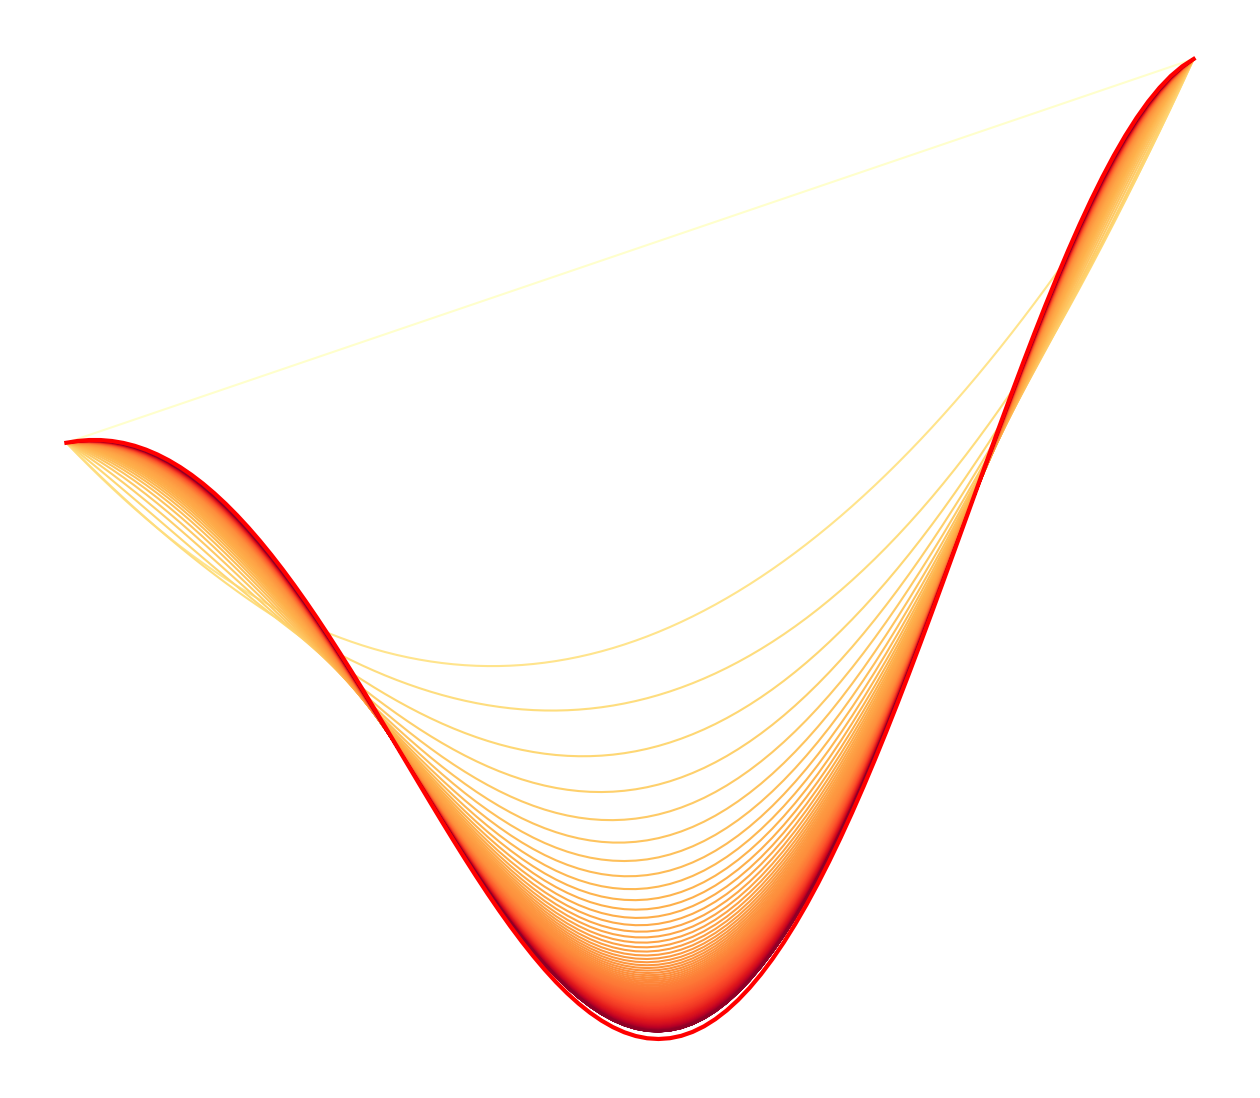
\includegraphics[width=0.9\textwidth]{./img/expansions.png}
            \label{fig:bernstein_expansion}
        \end{figure}
    \end{frame}

    \section{Generalizing polynomials}
    
    \begin{frame}{Algebras of functions}
        A collection of real valued functions $\mathscr{A}$ on a set $E$ is called an
        algebra if
        \begin{itemize}
            \item $f \in \mathscr{A}, g \in \mathscr{A} \implies f + g \in \mathscr{A}$
            \item $f \in \mathscr{A}, g \in \mathscr{A} \implies fg \in \mathscr{A}$
            \item $f \in \mathscr{A}, c \in \R \:\implies cf \in \mathscr{A}$
        \end{itemize}

        \\~\\

        If $f \in \mathscr{A}$ and $p$ is a polynomial, then $p\circ f \in
        \mathscr{A}$.
    \end{frame}

    \begin{frame}{Interpolation}
        An algebra $\mathscr{A}$ vanishes at no point of $E$ if given $x \in E$,
        there exists $f \in \mathscr{A}$ such that $f(x) \neq 0$.

        An algebra separates points of $E$ if given distinct $x_1, x_2 \in E$, there
        exists $f \in \mathscr{A}$ such that $f(x_1) \neq f(x_2)$.

        \\~\\

        Let the algebra $\mathscr{A}$ vanish at no point of $E$ and separate
        points of $E$. Given distinct $x_1, x_2 \in E$ and $c_1, c_2 \in \R$, there
        exists $f \in \mathscr{A}$ such that $f(x_1) = c_1$, $f(x_2) = c_2$.
    \end{frame}

    \begin{frame}{Interpolation}
        Let $f_1, f_2 \in \mathscr{A}$ such that $f_1(x_1) \neq 0$ and $f_2(x_2) \neq
        0$, and let $g \in \mathscr{A}$ such that $g(x_1) \neq g(x_2)$. Define the
        functions \[
            h_1 = \frac{g - g(x_2)}{g(x_1) - g(x_2)} \frac{f_1}{f_1(x_1)}, \qquad
            h_2 = \frac{g - g(x_1)}{g(x_2) - g(x_1)} \frac{f_2}{f_2(x_2)}.
        \] Note that $h_i(x_j) = \delta_{ij}$. Finally, set \[
            f = c_1 h_1 + x_2 h_2. \tag*{\qed}
        \] 

        \\~\\

        Note that this can be extended to arbitrarily many points, in the manner of
        Lagrange interpolation.
    \end{frame}
    
    \begin{frame}{Interpolation and continuity}
        Let $f$, $g$ be continuous, real valued functions on $X$ such that $f(x_0) =
        g(x_0)$ for some $x_0 \in X$. Then, $g$ approximates $f$ to an arbitrary
        degree of accuracy $\epsilon$ on some neighbourhood of $x_0$.

        \\~\\

        Note that $h = g - f$ is continuous, hence the pre-image of the open interval
        $(-\epsilon, +\epsilon)$ is some open set $U \subseteq X$ containing
        $x_0$. Thus, on some neighbourhood $N_\delta(x_0) \subseteq U$, we have \[
            -\epsilon < g - f < \epsilon
        \] \[
            f - \epsilon < g < f + \epsilon \tag*{\qed}
        \] 
    \end{frame}

    \begin{frame}{Closure}
        The set of uniform limits of functions from an algebra is called its uniform
        closure.
        
        \\~\\

        A uniformly closed algebra contains all uniform limits of its functions.

        \\~\\

        The uniform closure $\mathscr{B}$ of an algebra $\mathscr{A}$ of bounded
        functions is a uniformly closed algebra.
    \end{frame}
    
    \begin{frame}{Closure}
        Let $\mathscr{A}$ be an algebra of real valued, bounded functions on $X$, and
        let $\mathscr{B}$ be its uniform closure. If $f \in \mathscr{B}$, then $|f|
        \in \mathscr{B}$.

        \\~\\

        Let $\epsilon > 0$, let $M$ be such that $|f| < M$. Pick a polynomial $p$
        such that for all $|x| < M$, \[
            |p(x) - |x| | < \epsilon.
        \] Then, for all $x \in X$, we have $|f(x)| < M$ so \[
            |p(f(x)) - |f(x)| | < \epsilon.
        \] Finally, note that $p\circ f \in \mathscr{B}$. \hfill\qed
    \end{frame}

    \begin{frame}{Closure}
        If $f, g \in \mathscr{B}$, then $\max(f, g) \in \mathscr{B}$ and $\min(f, g)
        \in \mathscr{B}$.

        \\~\\

        Note that \[
            \max(f, g) = \frac{1}{2}(f + g) + \frac{1}{2}|f - g|,
        \] \[
            \min(f, g) = \frac{1}{2}(f + g) - \frac{1}{2}|f - g|. \tag*{\qed}
        \]

        \\~\\

        This gives us a way of `stitching' functions from $\mathscr{B}$ together.
    \end{frame}

    \section{The Stone-Weierstrass Theorem}

    \begin{frame}{The Stone-Weierstrass Theorem}
        Let $K$ be a compact metric space, and let $\mathscr{A}$ be an algebra of
        real continuous functions on $K$ which separates points of $K$ and vanishes
        at no point of $K$. The uniform closure of $\mathscr{A}$ consists of all real
        valued, continuous functions on $K$.

        \\~\\

        In other words, given any real valued continuous function $f$ on $K$, there
        exists a sequence of functions $\{f_n\}$ from $\mathscr{A}$ such that $f_n
        \to f$ uniformly on $K$.
    \end{frame}
    
    \newcounter{weierstrass_A_step}
    \begin{frame}
        \begin{figure}
            \begin{overprint}
            \forloop{weierstrass_A_step}{1}{\value{weierstrass_A_step} < 5} {
                \onslide<\arabic{weierstrass_A_step}>\centering\includegraphics[width=1.0\textwidth]{./img/weierstrass_A_\arabic{weierstrass_A_step}.png}
            }
            \end{overprint} 
        \end{figure}
        \begin{overprint}
        \onslide<1-3>\[
            f - \epsilon < g_{st} \qquad\text{ for all } x \in U_{st}
        \]
        \onslide<4>\[
            f - \epsilon < g_s \qquad\text{ for all } x \in K
        \]
        \end{overprint}
    \end{frame}
    
    \newcounter{weierstrass_B_step}
    \begin{frame}
        \begin{figure}
            \begin{overprint}
            \forloop{weierstrass_B_step}{1}{\value{weierstrass_B_step} < 5} {
                \onslide<\arabic{weierstrass_B_step}>\centering\includegraphics[width=1.0\textwidth]{./img/weierstrass_B_\arabic{weierstrass_B_step}.png}
            }
            \end{overprint} 
        \end{figure}
        \begin{overprint}
        \onslide<1-3>\[
            f - \epsilon < g_{s} < f + \epsilon \qquad\text{ for all } x \in U_{s}
        \]
        \onslide<4>\[
            f - \epsilon < g < f + \epsilon \qquad\text{ for all } x \in K \tag*{\qed}
        \]
        \end{overprint}
    \end{frame}
    
        
\end{document}
% vim: set tabstop=4 shiftwidth=4 softtabstop=4:
